\documentclass[11pt]{book}
\usepackage{palatino}
\usepackage{amsfonts,amsmath,amssymb}
% \usepackage{graphicx}


\ifx\pdftexversion\undefined
    \usepackage[dvips]{graphicx}
\else
    \usepackage[pdftex]{graphicx}
    \usepackage{epstopdf}
    \epstopdfsetup{suffix=}
\fi


\begin{document}

%%%%%%%%%%%%%%%%%%%%%%%%%%%%%%%%%%%%%%%%
% Problem Set 6
%%%%%%%%%%%%%%%%%%%%%%%%%%%%%%%%%%%%%%%%

\pagestyle{empty}
{\noindent\bf Spring 2021 \hfill Firstname M.~Lastname}
\vskip 16pt
\centerline{\bf University of Central Florida}
\centerline{\bf College of Business}
\vskip 16pt
\centerline{\bf QMB 6911}
\centerline{\bf Capstone Project in Business Analytics}
\vskip 10pt
\centerline{\bf Solutions:  Problem Set \#6}
\vskip 32pt
\noindent




\pagebreak
\section*{Probability Density Function of Fly Reel Prices}

Figure \ref{fig:density_prices} depicts
the kernel-smoothed probability density function of fly reel
prices.

\begin{figure}[h!]
  \centering
  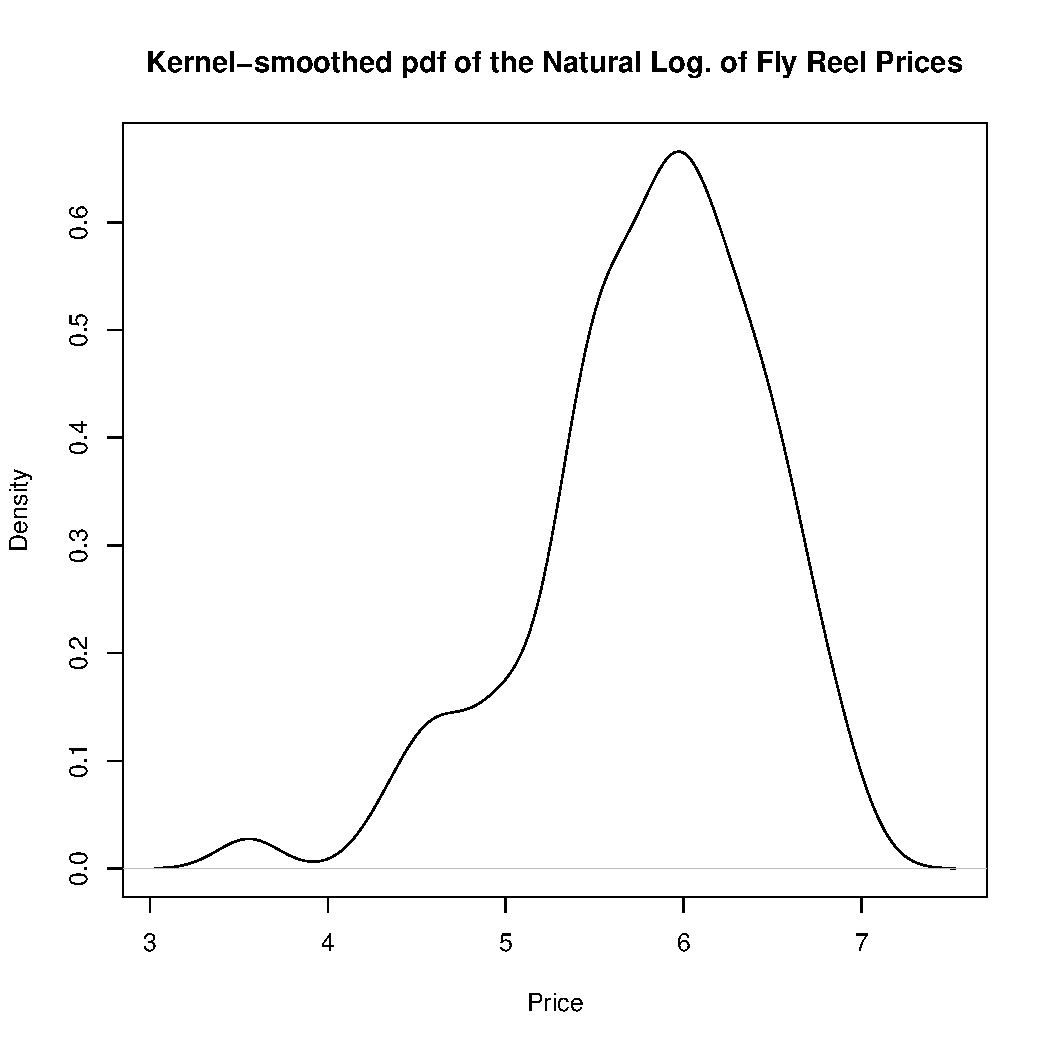
\includegraphics[scale = 0.5, keepaspectratio=true]{../Figures/density_prices}
  \caption{Probability Density Function of Fly Reel Prices} \label{fig:density_prices}
\end{figure}



\pagebreak
\section*{Probability Density Function of the Logarithm of Fly Reel Prices}

Figure \ref{fig:density_log_prices} depicts
the kernel-smoothed probability density function of the natural logarithm of fly reel
prices.

\begin{figure}[h!]
  \centering
  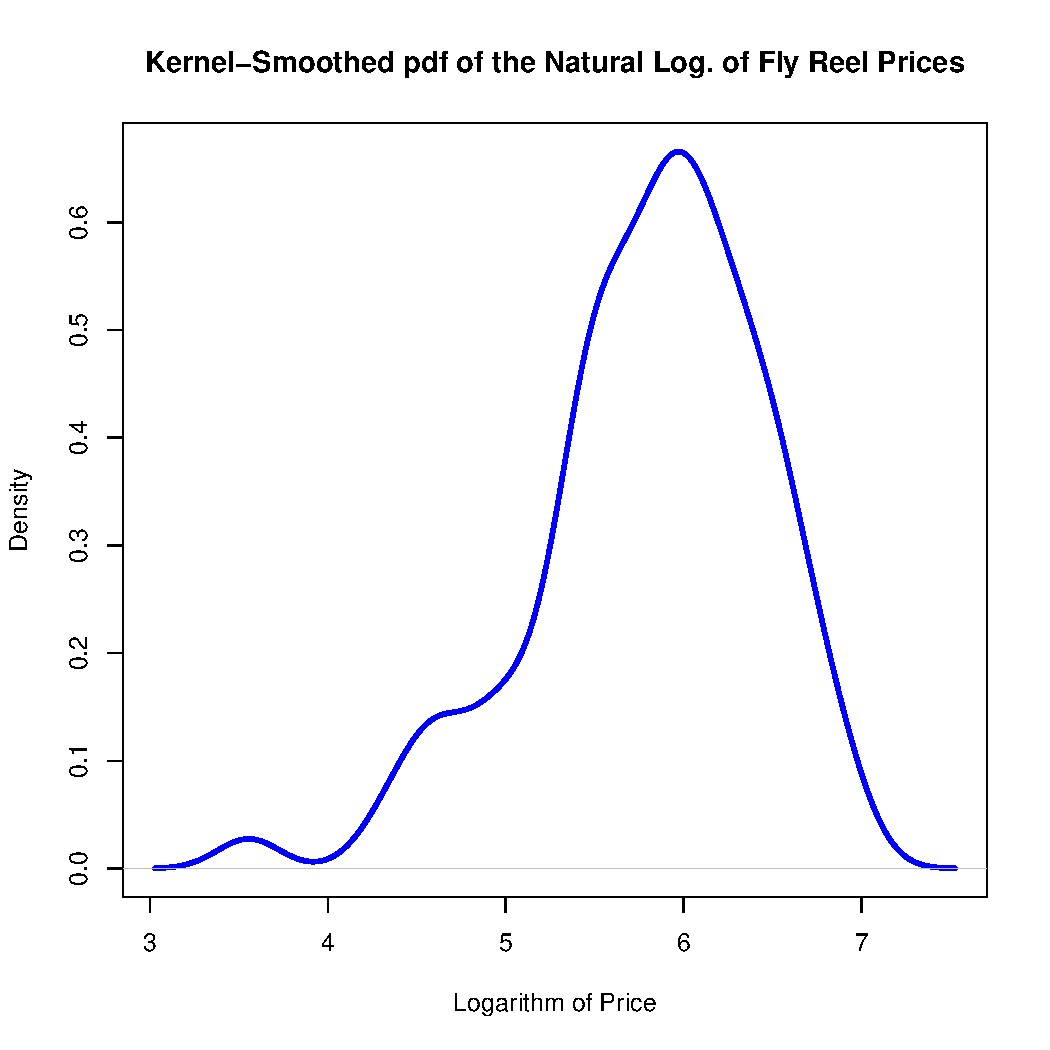
\includegraphics[scale = 0.5, keepaspectratio=true]{../Figures/density_log_prices}
  \caption{Probability Density Function of Fly Reel Prices} \label{fig:density_log_prices}
\end{figure}







%%%%%%%%%%%%%%%%%%%%%%%%%%%%%%%%%%%%%%%%
\end{document}
%%%%%%%%%%%%%%%%%%%%%%%%%%%%%%%%%%%%%%%%
